
\documentclass{standalone}
\usepackage{tikz}
\usepackage{adjustbox}
\usepackage{helvet}  
\usepackage{sansmathfonts}  
\renewcommand{\familydefault}{\sfdefault}  
\usetikzlibrary{arrows.meta,calc,decorations.pathmorphing}
\usetikzlibrary{shapes.arrows}
\usepackage{xcolor}
\definecolor{color001122}{HTML}{001122}
\definecolor{colorf0f0ff}{HTML}{f0f0ff}
\definecolor{color354a7b}{HTML}{354a7b}
\definecolor{color00caff}{HTML}{00caff}
\begin{document}
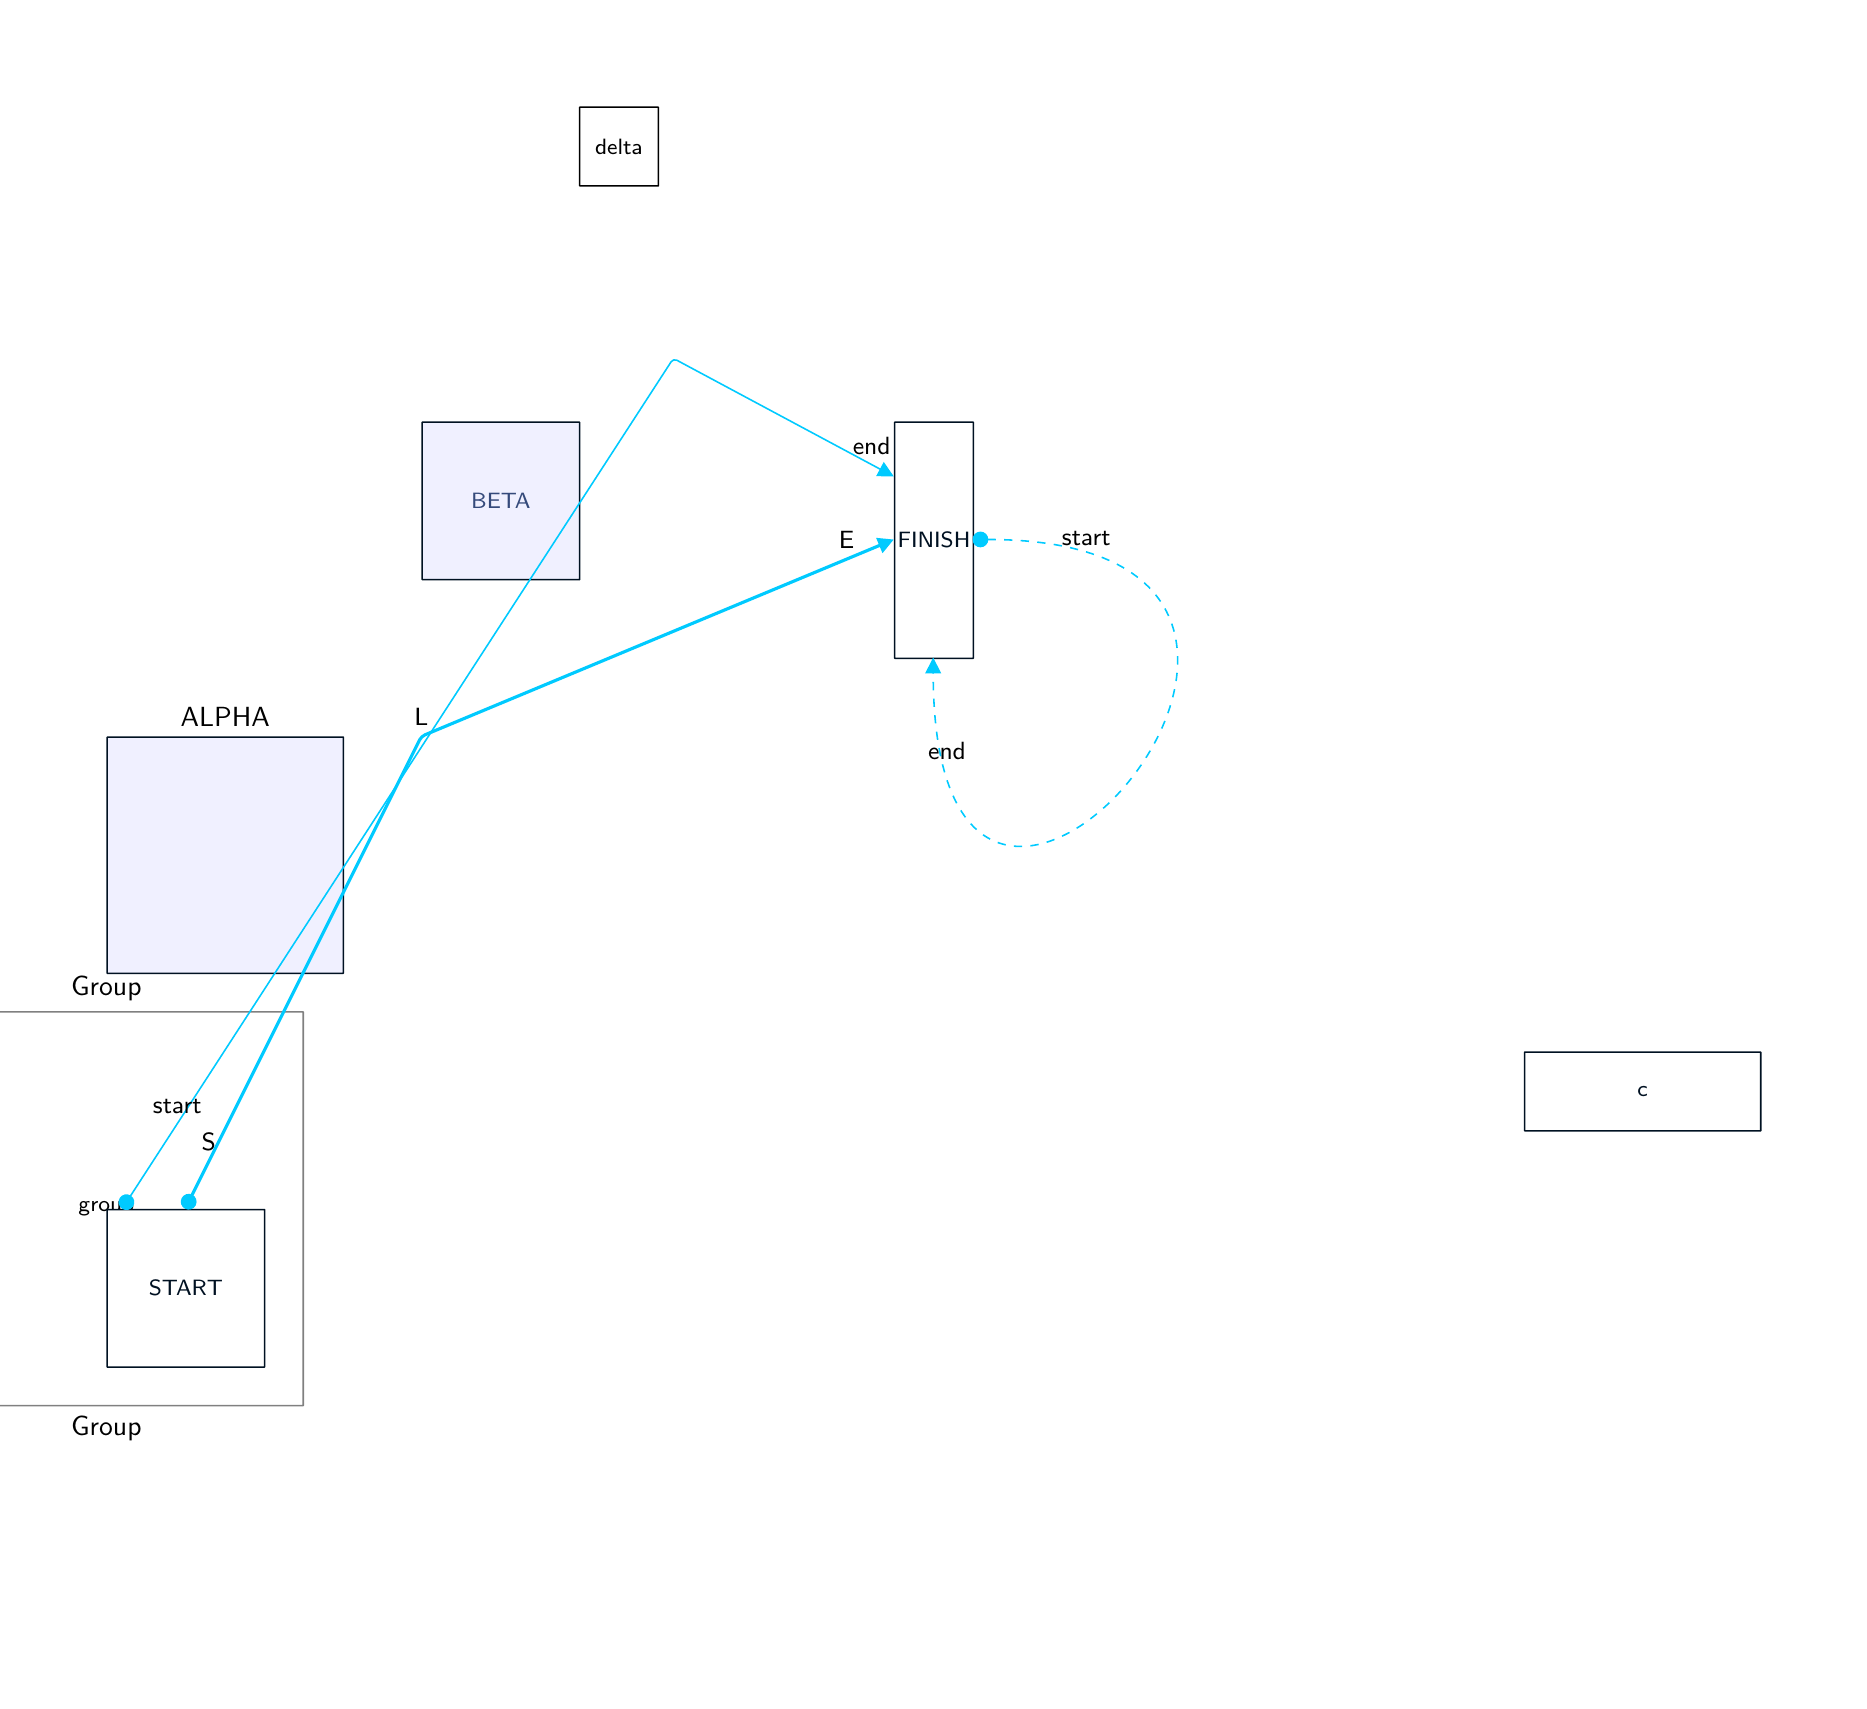
\begin{tikzpicture}
    [>={Stealth[scale=1.0]},  % Uniform arrow style
    ]
     \useasboundingbox (3,-2) rectangle (26,19);
    
\node[shape=rectangle, fill=white, draw=gray, minimum width=5cm, minimum height=5cm, rounded corners=0.005cm, line width=0.02cm, text opacity=1, font=\footnotesize, inner sep=0pt,label=above:{Group},label=below:{Group}] (node_group) at (4,4) {\adjustbox{max width=5cm, max height=5cm}{group}};
\node[shape=rectangle, anchor=north west, fill=white, draw=color001122, minimum width=2cm, minimum height=2cm, rounded corners=0.005cm, line width=0.02cm, text opacity=1, font=\footnotesize, inner sep=0pt] (node_a) at (4,4) {\adjustbox{max width=2cm, max height=2cm}{\textcolor{color001122}{START}}};
\node[shape=rectangle, anchor=north west, fill=white, draw=color001122, minimum width=1cm, minimum height=3cm, rounded corners=0.005cm, line width=0.02cm, text opacity=1, font=\footnotesize, inner sep=0pt] (node_b) at (14,14) {\adjustbox{max width=1cm, max height=3cm}{\textcolor{color001122}{FINISH}}};
\node[shape=rectangle, anchor=north west, fill=white, draw=color001122, minimum width=3cm, minimum height=1cm, rounded corners=0.005cm, line width=0.02cm, text opacity=1, font=\footnotesize, inner sep=0pt] (node_c) at (22,6) {\adjustbox{max width=3cm, max height=1cm}{\textcolor{color001122}{c}}};
\node[shape=rectangle, anchor=north west, fill=colorf0f0ff, draw=color001122, minimum width=3cm, minimum height=3cm, rounded corners=0.005cm, line width=0.02cm, text opacity=1, font=\footnotesize, inner sep=0pt,label=above:{ALPHA}] (node_alpha) at (4,10) {\adjustbox{max width=3cm, max height=3cm}{\textcolor{color001122}{ }}};
\node[shape=rectangle, anchor=north west, fill=colorf0f0ff, draw=color001122, minimum width=2cm, minimum height=2cm, rounded corners=0.005cm, line width=0.02cm, text opacity=1, font=\footnotesize, inner sep=0pt] (node_beta) at (8,14) {\adjustbox{max width=2cm, max height=2cm}{\textcolor{color354a7b}{BETA}}};
\node[shape=rectangle, anchor=north west, fill=white, draw=black, minimum width=1cm, minimum height=1cm, rounded corners=0.005cm, line width=0.02cm, text opacity=1, font=\footnotesize, inner sep=0pt] (node_delta) at (10,18) {\adjustbox{max width=1cm, max height=1cm}{delta}};
\draw[draw=color00caff, line width=0.02cm, rounded corners=0.05cm, dashed, arrows={Circle[width=0.2cm,length=0.2cm]}-{Triangle[width=0.2cm,length=0.2cm]}] (15,12.5) .. controls (21,12.5) and (14.5,5) .. (14.5,11) node[above, pos=0.1] {\small{\sffamily{start}}} node[above, pos=0.9] {\small{\sffamily{end}}};
\draw[draw=color00caff, line width=0.04cm, rounded corners=0.05cm, arrows={Circle[width=0.2cm,length=0.2cm]}-{Triangle[width=0.2cm,length=0.2cm]}] (5,4) -- (8,10) node[above, pos=0.1] {\small{\sffamily{S}}} -- (14,12.5) node[above, pos=0.9] {\small{\sffamily{E}}} node[above, pos=0] {\small{\sffamily{L}}};
\draw[draw=color00caff, line width=0.02cm, rounded corners=0.05cm, arrows={Circle[width=0.2cm,length=0.2cm]}-{Triangle[width=0.2cm,length=0.2cm]}] (4.2,4) -- (11.2,14.8) node[above, pos=0.1] {\small{\sffamily{start}}} -- (14,13.3) node[above, pos=0.9] {\small{\sffamily{end}}};

\end{tikzpicture}
\end{document}
